\part{Introduction}
\chapter{Introduction}\label{ch:introduction}

This is a technical research paper covering the scientific part of the development 
of the open-source MoleHole project\footnote{\url{https://github.com/g-martin772/MoleHole}}. 
It is not a user manual, neither a tutorial, and it is not particularly intended to be read linearly.
This paper aims to cover both the very foundational concepts of computer graphics, physics and mathematics,
as well as highly specific technical details about general relativistic ray tracing and physical simulations.
The reader is encouraged to read the table of contents first and jump between sections of interest.

\section{Motivation}\label{sec:motivation}

Inspired by the visual display of the black hole \emph{Gargantua} in the movie \emph{Interstellar}\cite{Nolan2014Interstellar},
and a general interest in computer graphics and physics, we decided to build a black hole simulator.
What started as a simple school project soon evolved into a more ambitious project,
aiming to create an interactive application able to export physically accurate renderings
of black holes and other stellar objects.

For \emph{Interstellar}, the visual effects company ``Double Negative'' developed the \gls{dngr},
which traces bundles of light rays through the spacetime of a spinning black hole instead individual ones\cite{James15}.
The spin was lowered from $a/M = 0.999$ to $a/M = 0.6$ 
because the flattened shadow edge and multiple disk images
were deemed too confusing for a general audience\cite{James15}.
The same code was later used for scientific publications.
For example the visualization of the movie's wormhole\cite{James15b}.

In 2019 the \gls{eht}, 
a global network of radio telescopes combined through \gls{vlbi} at a wavelength of \SI{1.3}{\milli\metre},
published the first image of the supermassive black hole M87*\cite{EHT19}.
In 2022 the image of Sagittarius~A*, the black hole at the center of the Milky Way Galaxy\cite{EHT22}.
\Cref{fig:motivation-images} shows these images next to the \gls{dngr} rendering.

\begin{figure*}[t]
    \centering
    \begin{subfigure}[t]{0.49\textwidth}
        \centering
        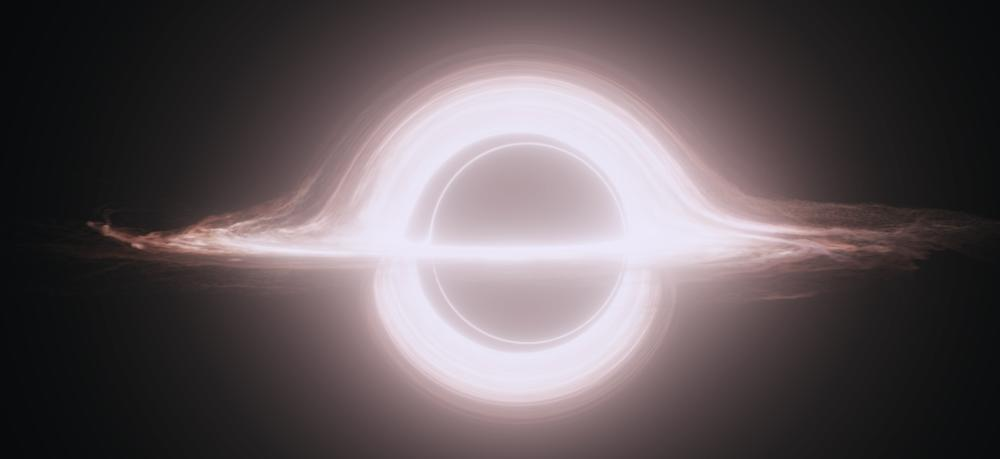
\includegraphics[height=3.6cm]{intro/gargantua-dngr.jpg}
        \caption{\emph{Interstellar} (\gls{dngr}), $a/M = 0.6$}
    \end{subfigure}\hfill
    \begin{subfigure}[t]{0.27\textwidth}
        \centering
        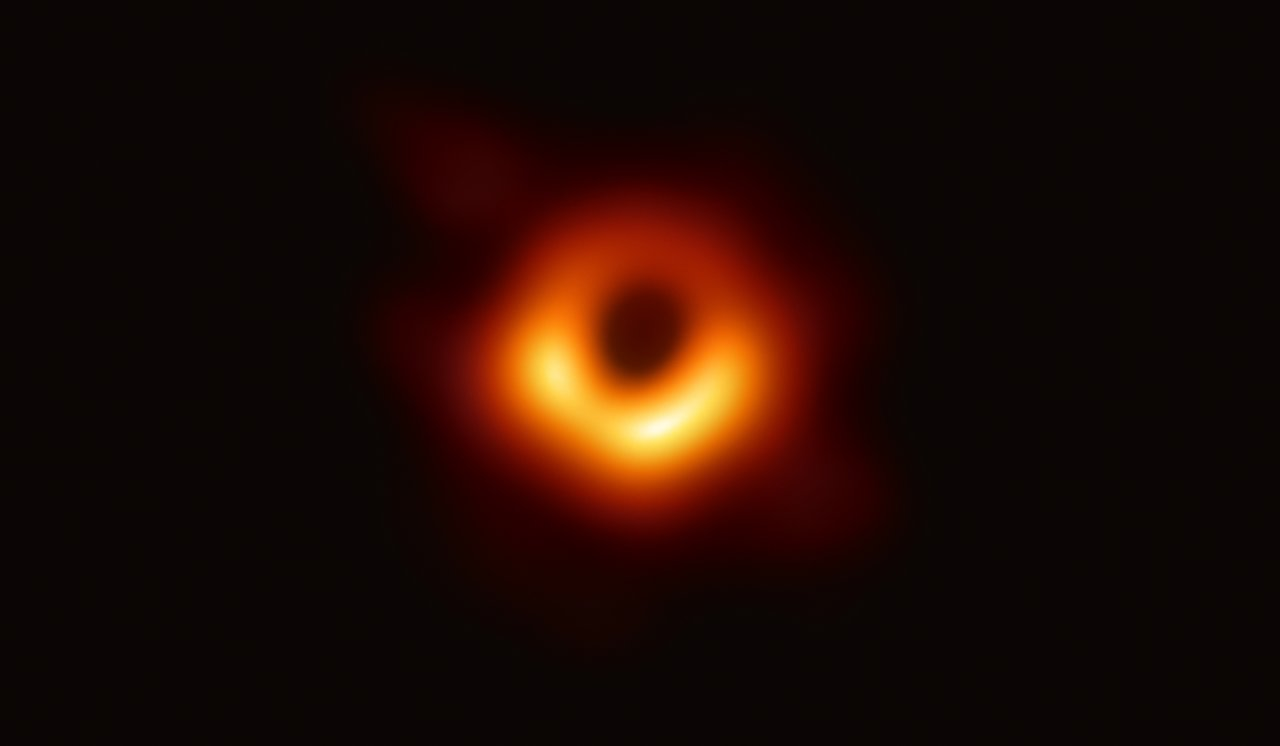
\includegraphics[height=3.6cm, trim=300 66 300 60, clip]{intro/m87-eht-2019.jpg}
        \caption{M87*, \gls{eht} 2017}
    \end{subfigure}\hfill
    \begin{subfigure}[t]{0.23\textwidth}
        \centering
        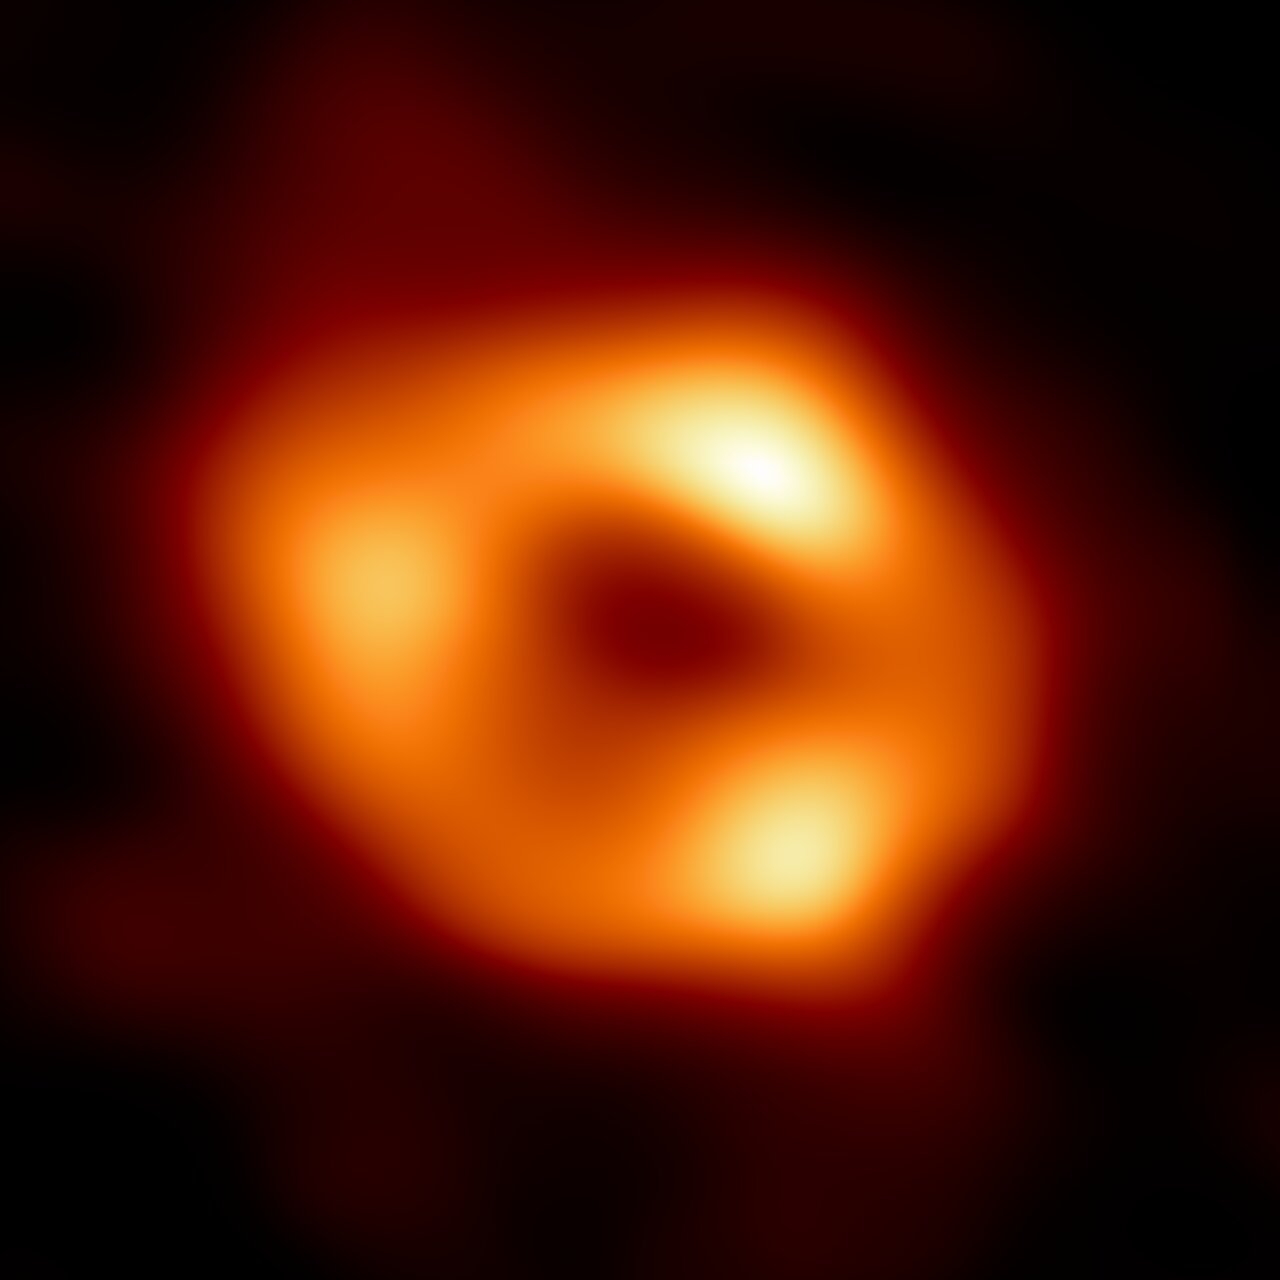
\includegraphics[height=3.6cm]{intro/sgra-eht-2022.jpg}
        \caption{Sgr~A*, \gls{eht} 2022}
    \end{subfigure}
    \caption{A simulated and two observed black hole images.
    (a)~Rendered with \gls{dngr}. A variant of the disk seen in \emph{Interstellar}\cite{James15}.
    (b)~M87*\cite{EHT19}
    (c)~Sagittarius~A*\cite{EHT22}
    \label{fig:motivation-images}}
\end{figure*}


\section{Related Work}\label{sec:related-work}
\planned{DNGR, GYOTO, GRay, RAPTOR, geokerr, GeodesicViewer, Riazuelo}

\section{Problem Statement and Contributions}\label{sec:problem-statement-and-contributions}
\planned{what is new, tiered renderer, spectral $g$-shifted transfer, Kerr--Schild orientation}

\section{Outline and Reading Paths}\label{sec:outline-and-reading-paths}
\planned{prerequisites, rendering reader vs. physics reader}

\section{Notation and Conventions}\label{sec:notation-and-conventions}
\planned{signature $(-+++)$, $G=c=1$, index conventions}


\part{Mathematical Foundations}
\chapter{Space and Coordinates}\label{ch:coordinates}

This chapter revises the basic concepts of common coordinate systems and their use in computer graphics. 
It also covers specific implementation details and conventions for representing vectors, transformations,
and other data structures in C/C++ and Vulkan/GLSL. 

This chapter assumes you are already familiar with the basic concepts of linear algebra, 
including vectors and matrices, trigonometry, and basic calculus.

\section{Common Coordinate Systems}\label{sec:common-coordinate-systems}

In simple terms, a coordinate system is a $1:1$ mapping from a geometric space $S$ to a set of real numbers $\mathbb{R}^n$.
It has a fixed origin or reference point, often defines a set of basis vectors also called axes, 
and defines a set of units or parameters to express the coordinates of a point in this space
(e.g. linear distances or angular  measurements).  
This section covers the most common coordinate systems and common operations on them\cite{arfken2012mathematical}.

\subsection{Cartesian Coordinates}\label{subsec:cartesian-coordinates}

Defined by a set of perpendicular axes, Cartesian coordinates are the most common system used to represent Euclidean geometry. 
It is widely used in everyday life, CAD, and physics.
It typically uses two or three dimensions, with the origin at the intersection of the axes.
The coordinates of a point are expressed as $(x,y)$ in 2D or $(x,y,z)$ in 3D, 
where $x$ (horizontal), $y$ (vertical), and $z$ (depth) are the linear distances from the origin along the respective axes. 

For any two points $P_1=(x_1,y_1,z_1)$ and $P_2=(x_2,y_2,z_2)$, 
the Euclidean distance between them is given by $d$:
\[
d(P_1,P_2)=\sqrt{(x_2-x_1)^2+(y_2-y_1)^2+(z_2-z_1)^2}
\]

Given two vectors $\mathbf{a}$ and $\mathbf{b}$, the dot product represents the cosine of the angle between them,
while the cross product represents a vector perpendicular to both.

\[
\mathbf{a}\cdot\mathbf{b} = |\mathbf{a}||\mathbf{b}|\cos\theta
\]
\[
\mathbf{a}\times\mathbf{b} = |\mathbf{a}||\mathbf{b}|\sin\theta \, \mathbf{n}
\]

The determinant of a $3\times 3$ matrix formed by three vectors $\mathbf{a}$, $\mathbf{b}$, and $\mathbf{c}$ 
gives the volume of the parallelepiped between them\cite{strang2016introduction,stewart2020calculus}:

\[
V = \det(\mathbf{a},\mathbf{b},\mathbf{c})
\]

To transform (translate, scale, and rotate) a point/vector in 3D space, 
a $4\times 4$ transformation matrix can be used. See Figure~\ref{eq:transformation-matrix}.
Note that the order of operations for matrix multiplication is not commutative.~\cite{strang2016introduction}

\begin{figure*}[!t]
\begin{align}
M_{\text{translate}} &= 
\begin{bmatrix} 
    1 & 0 & 0 & t_x \\ 0 & 1 & 0 & t_y \\ 0 & 0 & 1 & t_z \\ 0 & 0 & 0 & 1 
\end{bmatrix}
\\
M_{\text{scale}} &= 
\begin{bmatrix} 
    s_x & 0 & 0 & 0 \\ 0 & s_y & 0 & 0 \\ 0 & 0 & s_z & 0 \\ 0 & 0 & 0 & 1 
\end{bmatrix}
\\
M_{\text{rotate}} &= 
\begin{bmatrix} 
    \cos\alpha\cos\beta & \cos\alpha\sin\beta\sin\gamma - \sin\alpha\cos\gamma & \cos\alpha\sin\beta\cos\gamma + \sin\alpha\sin\gamma & 0 \\ 
    \sin\alpha\cos\beta & \sin\alpha\sin\beta\sin\gamma + \cos\alpha\cos\gamma & \sin\alpha\sin\beta\cos\gamma - \cos\alpha\sin\gamma & 0 \\ 
    -\sin\beta & \cos\beta\sin\gamma & \cos\beta\cos\gamma & 0 \\ 
    0 & 0 & 0 & 1 
\end{bmatrix}
\end{align}
\caption{Transformation matrices for Cartesian coordinates}
\label{eq:transformation-matrix}
\end{figure*}

\subsection{Polar Coordinates}\label{subsec:polar-coordinates}

A point in 2D polar coordinates is expressed as $(r,\theta)$,
where $r$ is the radial distance from the origin and $\theta$ is the angle measured counterclockwise from the positive $x$-axis.
The conversion between Cartesian and polar coordinates: 
$x = r\cos\theta$, $y = r\sin\theta$ and $r = \sqrt{x^2+y^2}$, $\theta = \arctan2(y,x)$.~\cite{arfken2012mathematical}

Polar coordinates are commonly used in physics and engineering for problems with circular symmetry, such as wave propagation.
They are also the basis for imaginary numbers and complex analysis, 
where a complex number $z$ can be represented as $z = re^{i\theta}$.

\subsection{Spherical Coordinates}\label{subsec:spherical-coordinates}

Similar to polar coordinates, a point in 3D spherical coordinates is expressed as $(r,\theta,\phi)$,
where $r$ is the radial distance from the origin, $\theta$ is the polar angle measured from the positive $z$-axis,
and $\phi$ is the azimuthal angle measured counterclockwise from the positive $x$-axis in the $xy$-plane.
See Figure~\ref{fig:spherical-coordinates}.
The conversion between Cartesian and spherical coordinates:
$x = r\sin\theta\cos\phi$,  $y = r\sin\theta\sin\phi$, $z = r\cos\theta$, and
$r = \sqrt{x^2+y^2+z^2}$, $\theta = \arccos(z/r)$, $\phi = \arctan2(y,x)$.~\cite{arfken2012mathematical}

\begin{figure}[htbp]
    \centering
    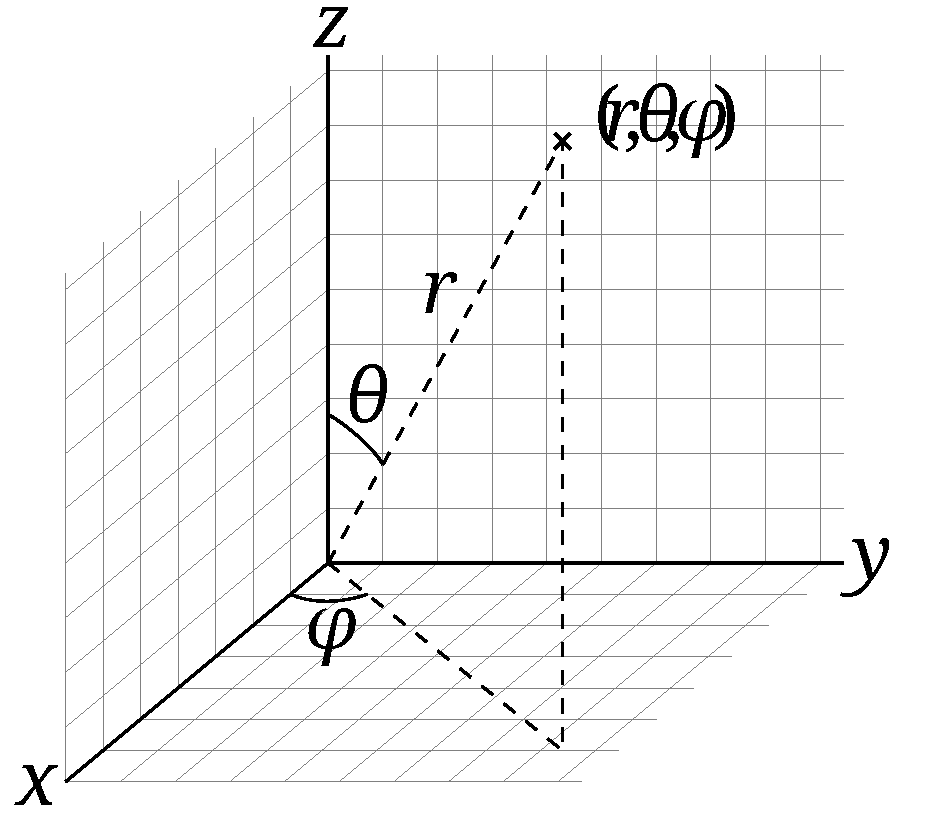
\includegraphics[width=0.75\columnwidth]{coordinates/3D_Spherical} 
    \caption{3D Spherical Coordinate System representation.}
    \label{fig:spherical-coordinates}
\end{figure}

\subsection{Schwarzschild Coordinates}\label{subsec:schwarzschild-coordinates}
\subsection{Eddington-Finkelstein Coordinates}\label{subsec:einstein-finkelstein-coordinates}
\subsection{Kruskal-Szekeres Coordinates}\label{subsec:kruskal-szekeres-coordinates}
\subsection{Painlevé-Gullstrand Coordinates}\label{subsec:painleve-gullstrand-coordinates}
\subsection{Boyer-Lindquist  Coordinates}\label{subsec:boyer-lindquist-coordinates}
\subsection{Kerr-Schild Coordinates}\label{subsec:kerr-schild-coordinates}
\subsection{Penrose Coordinates}\label{subsec:penrose-coordinates}


\section{The Jacobian}\label{sec:jacobian}

In multivariable calculus, 
the Jacobian is the basic mathematical framework for linearizing vector-valued functions 
and transforming coordinate systems. 
Depending on the context, the term Jacobian refers to either the matrix 
of first-order partial derivatives or to its corresponding determinant.~\cite{stewart2020calculus}

\subsection{The Jacobian Matrix}\label{subsec:jacobian-matrix}

The Jacobian matrix, 
denoted as $\mathbf{J}$ or $\frac{\partial(f_1, \dots, f_m)}{\partial(x_1, \dots, x_n)}$, 
is an $m \times n$ matrix of all possible first-order partial derivatives of $\mathbf{f}$. 
Each row corresponds to an output component function, and each column corresponds to an input variable:
\begin{equation}
    \mathbf{J} = \begin{pmatrix}
        \frac{\partial f_1}{\partial x_1} & \frac{\partial f_1}{\partial x_2} & \cdots & \frac{\partial f_1}{\partial x_n} \\
        \frac{\partial f_2}{\partial x_1} & \frac{\partial f_2}{\partial x_2} & \cdots & \frac{\partial f_2}{\partial x_n} \\
        \vdots & \vdots & \ddots & \vdots \\
        \frac{\partial f_m}{\partial x_1} & \frac{\partial f_m}{\partial x_2} & \cdots & \frac{\partial f_m}{\partial x_n}
    \end{pmatrix}
\end{equation}

Geometrically, 
the Jacobian matrix represents the best linear approximation of the function $\mathbf{f}$ 
in near a given point $\mathbf{p}$. 
It is the multivariable version of the single-variable derivative $f'(x)$.

\subsection{The Jacobian Determinant}
When a vector-valued function maps space to a space of the same dimension ($m = n$), 
the Jacobian matrix is a square. 
We can then compute its determinant:
\begin{equation}
    \det(\mathbf{J}) = \left| \frac{\partial(f_1, \dots, f_n)}{\partial(x_1, \dots, x_n)} \right|
\end{equation}

The Jacobian determinant represents the local \textit{space-scaling factor} of the transformation. 
It quantifies how much a small, differential volume or area expands, contracts, or flips orientation 
when processed through the function $\mathbf{f}$ at a specific location.

\subsection{Application: Change of Variables}
The primary analytical application of the Jacobian determinant is modifying boundaries and differentials 
during multivariable integration. (Change of variables theorem, used later).
When transitioning from a coordinate system $(x,y)$ to an alternative system $(u,v)$ via the transformations $x = x(u,v)$ 
and $y = y(u,v)$, the differential area element scales based on the absolute value of the Jacobian determinant:
\begin{equation}
    dx \, dy = \left| \det(\mathbf{J}) \right| du \, dv = \left| \frac{\partial x}{\partial u}\frac{\partial y}{\partial v} - \frac{\partial x}{\partial v}\frac{\partial y}{\partial u} \right| du \, dv
\end{equation}

Therefore, a double integral over a Cartesian region $R$ 
translates over a mapped region $G$ under the new coordinates as:
\begin{align}
    &\iint_R f(x, y) \, dx \, dy = \\
    &\iint_G f(x(u,v), y(u,v)) \left| \frac{\partial(x, y)}{\partial(u, v)} \right| du \, dv
\end{align}




\section{Calculus in Curvilinear Coordinates}\label{sec:calculus-in-curvilinear-coordinates}
\planned{$\nabla$, solid angle $\mathrm{d}\Omega=\sin\theta\,\mathrm{d}\theta\,\mathrm{d}\phi, \int_{\Omega}$}

\section{Rotations and Orientation}\label{sec:rotations-and-orientation}
\planned{$SO(3)$, axis--angle, Euler, quaternions, slerp, aligning a spin axis to $+z$}

\section{Homogeneous Coordinates and Projection}\label{sec:homogeneous-coordinates-and-projection}
\planned{affine maps, pinhole, NDC, camera-relative origin, perspective projection matrix, view matrix, model matrix}

\section{The Celestial Sphere\optmark}\label{sec:the-celestial-sphere}
\planned{equirectangular, cubemap, sampling distortion, HEALPix}


\section{Computer Hardware Limitations and Screen Space Conventions}\label{sec:computer-hardware-limitations-and-screen-space-conventions}

This section covers basic memory alignment and data layouts in C/C++ and GLSL, 
and compares the conventions used by different graphics APIs, programming languages, and hardware limitations.

\subsection{Memory Layouts and conventions}\label{subsec:memory-layouts}

The C and C++ compiler automatically aligns data structures in memory to optimize access speed.
\TODO{C compiler reference}

On the GPU side, the Vulkan specification defines three different memory layouts: 
\texttt{std140}, \texttt{std430}, and \texttt{scalar}. See Table~\ref{tab:memory-layouts} for a direct comparison.


\begin{table*}[htbp]
\centering
\caption{Direct Comparison of Vulkan Buffer Memory Layouts}
\label{tab:memory-layouts}
\begin{tabular}{p{4.4cm} p{3.6cm} p{3.6cm} p{3.6cm}}
\hline
\textbf{Feature / Member Type} & \textbf{\texttt{std140} (Extended)} & \textbf{\texttt{std430} (Base)} & \textbf{\texttt{scalar} (Scalar)} \\ \hline
\textbf{Primary Use Case} & Default for Uniform Buffer Objects (UBOs). & Default for Shader Storage Buffer Objects (SSBOs). & Highly dense, tightly packed structures. \\
\textbf{Vulkan Core Status} & Standard core behavior. & Core since Vulkan 1.2 (via standard layout extension). & Core since Vulkan 1.2 (via scalar block layout). \\
\textbf{Scalars (\texttt{float}, \texttt{int})} & Aligned to base size (4 bytes). & Aligned to base size (4 bytes). & Tightly packed to base size (4 bytes). \\
\textbf{Vectors (\texttt{vec2}, \texttt{vec4})} & \texttt{vec2} = 8B; \texttt{vec3}/\texttt{vec4} = 16B alignment. & \texttt{vec2} = 8B; \texttt{vec3}/\texttt{vec4} = 16B alignment. & Aligned to component base size (\texttt{vec3} takes 12B). \\
\textbf{Array Element Stride} & Rounded up to a multiple of a \texttt{vec4} (\textbf{16 bytes}). & Equal to the base alignment of the element type. & Equal to the exact size of the element type. \\
\textbf{Nested Struct Alignment} & Rounded up to a multiple of \textbf{16 bytes}. & Aligned to its largest member's alignment. & Aligned to the alignment of its single largest scalar element. \\
\textbf{Memory Efficiency} & \textbf{Low}: Prone to heavy padding and wasted bandwidth. & \textbf{Medium}: Efficient for arrays, but \texttt{vec3} still pads. & \textbf{Maximum}: Zero padding; matches native C/C++ packaging. \\ \hline
\end{tabular}
\end{table*}



\TODO{row vs column major order}

\TODO{host visible/coherent and PICe bus + VRAM vs UM}

\TODO{rebar}

\subsection{Screen Space}\label{subsec:screen-space}

Different graphics APIs use different conventions for screen space coordinates.
OpenGL and Vulkan use normalized device coordinates (NDC) in the range $[-1, 1]$ for both $x$ and $y$ axes
($[0, 0]$ at the center of the screen),
while Direct3D uses the range $[0, 1]$ for the $y$ axis
($[0, 0]$ at the bottom-left corner of the screen).
While Vulkan defines the origin of the screen space at the top-left corner ($+X$ right, $+Y$ down), 
OpenGL defines the origin at the bottom-left corner ($+X$ right, $+Y$ up).


\chapter{Calculus, Variational Principles, Linear Algebra}\label{ch:calculus}
\plannedscope{The analysis that geodesics and Hamiltonians rest on}

\section{Taylor Series and Asymptotics}\label{sec:taylor-series-and-asymptotics}
\planned{big-O, order of approximation, weak-field expansions}

\section{Multivariable Calculus}\label{sec:multivariable-calculus}
\planned{chain rule, Jacobian, Hessian, change of variables, implicit function theorem}

\section{Singular Integrals}\label{sec:singular-integrals}
\planned{turning-point $1/\sqrt{\cdot}$ singularity, substitutions}

\section{Ordinary Differential Equations}\label{sec:ordinary-differential-equations}
\planned{IVP, Picard--Lindel\"of, autonomous systems, first integrals, phase space, stability}

\section{Calculus of Variations}\label{sec:calculus-of-variations}
\planned{Euler--Lagrange, Fermat's principle, Lagrangian mechanics, Noether and conserved quantities}

\section{Hamiltonian Mechanics}\label{sec:hamiltonian-mechanics}
\planned{Legendre transform, Hamilton's equations, Poisson bracket, Liouville theorem, Hamilton--Jacobi}

\section{Linear Algebra}\label{sec:linear-algebra}
\planned{inner products, eigen/SVD, Gram--Schmidt, indefinite inner products, $4\times4$ inverse and determinant}

\section{Special Functions and Polynomial Roots\optmark}\label{sec:special-functions-and-polynomial-roots}
\planned{elliptic integrals (Legendre, Carlson), Jacobi functions, cubic/quartic roots for ISCO and radial potential}

\chapter{Differential Geometry and Tensor Calculus}\label{ch:tensors}
\plannedscope{Everything needed to read the geodesic equation}

\section{Intuition: Intrinsic vs. Extrinsic Curvature}\label{sec:intuition-intrinsic-vs-extrinsic-curvatu}
\planned{the 2-sphere as running example}

\section{Manifolds and Charts}\label{sec:manifolds-and-charts}
\planned{atlases, coordinate transformations, why the sphere needs two charts}

\section{Tangent Vectors}\label{sec:tangent-vectors}
\planned{curves, directional derivatives, coordinate basis $\partial_\mu$}

\section{Covectors and One-Forms}\label{sec:covectors-and-one-forms}
\planned{dual basis, contra- vs. covariant}

\section{Tensors}\label{sec:tensors}
\planned{transformation law, products, contraction, symmetry, Einstein summation}

\section{The Metric}\label{sec:the-metric}
\planned{line element, signature, raising/lowering, $\sqrt{|g|}$, null/time/space-like, causal structure}

\section{Connection and Covariant Derivative}\label{sec:connection-and-covariant-derivative}
\planned{why $\partial$ fails, Christoffel symbols, metric compatibility}

\section{Parallel Transport and Geodesics}\label{sec:parallel-transport-and-geodesics}
\planned{variational and autoparallel derivations, affine parameter, null geodesics}

\section{Curvature}\label{sec:curvature}
\planned{Riemann, geodesic deviation, Ricci, Einstein, Weyl, Kretschmann, coordinate vs. true singularity, Bianchi}

\section{Killing Vectors and Conserved Quantities}\label{sec:killing-vectors-and-conserved-quantities}
\planned{Killing vectors and tensors, Lie derivative, conserved quantities along geodesics}

\section{Frame Fields and Tetrads}\label{sec:frame-fields-and-tetrads}
\planned{orthonormal frames, local Lorentz frame, spin connection}

\section{Hamiltonian Formulation on a Manifold}\label{sec:hamiltonian-formulation-on-a-manifold}
\planned{$H=\tfrac12 g^{\mu\nu}p_\mu p_\nu$, covariant momenta, symplectic structure}

\section{Differential Forms and Advanced Tools\optmark}\label{sec:differential-forms-and-advanced-tools}
\planned{exterior derivative, Cartan structure equations, Newman--Penrose, Petrov types}

\section{Worked Examples}\label{sec:worked-examples}
\planned{flat space in spherical coordinates ($\Gamma\neq0$ but $R=0$), 2-sphere, hyperbolic plane, embedding diagrams}

\chapter{Numerical Computation}\label{ch:numerics}
\plannedscope{What the machine does to our equations}

\section{Integers and Overflow}\label{sec:integer-overflows}

Discrete quantities are represented as binary signed or unsigned integers,
which can overflow when their values exceed the maximum or minimum representable values.
The range of an $n$-bit signed integer is $[-2^{n-1}, 2^{n-1}-1]$,
while an unsigned integer has a range of $[0, 2^n-1]$.

When an integer exceeds its maximum value, it wraps around to the minimum value (and vice versa).
Therefore, it is crucial to use sufficiently large integer types and/or implement overflow checking mechanisms.
This requires careful consideration of expected number ranges.



\section{Floating-Point Representation and Numerical Errors}\label{sec:floating-point}

Computers approximate real numbers using finite-precision representations 
governed by the IEEE 754 standard for floating-point arithmetic\cite{IEEE754_2019}.
Compared to integer representations, floating-point numbers can represent a much wider range of values,
by using a normalized scientific notation with a fixed number of significant digits (the mantissa) and an exponent.

Floating-point systems introduce fundamental error sources\cite{Goldberg1991FloatingPoint}:
\begin{itemize}
\item \textbf{Rounding and Machine Epsilon:} 
    Real numbers cannot be represented with infinite precision. 
    The spacing between adjacent representable floating-point numbers is bounded by the Machine Epsilon $\epsilon_{\text{mach}}$.
    Operations on physical quantities introduce rounding errors that accumulate over multistep time integrations 
    (e.g., Verlet or Runge-Kutta integrators).
    While single precision (32-bit) is the de facto standard for most programming languages, 
    it is insufficient for large-scale simulations with both high number ranges and small deltas.
    Double precision (64-bit) and quadruple precision (128-bit) are also available on modern processors, 
    but come with increased memory usage and computational cost. 
    See \Cref{tab:floating_point_comparison} for a comparison of IEEE 754 formats.
\item \textbf{Catastrophic Cancellation:}
    Subtracting two nearly equal floating-point numbers results in loss of significant digits. 
    This frequently occurs when computing relative position vectors between close particles 
    ($\vec{r}_1 - \vec{r}_2$), leading to increased relative errors.
\item \textbf{Underflow, Overflow, and NaN:}
    Exceeding the dynamic range of the exponent field results in overflow (yielding $\pm\infty$) 
    or underflow (yielding subnormal numbers or zero), which can corrupt calculations.
    A floating-point values might also hold the special value NaN (Not a Number) to indicate undefined or unrepresentable results,
    such as $0/0$ or $\infty - \infty$.
\end{itemize}

\begin{table*}
\centering
\small
\caption{Comparison of IEEE 754 floating-point formats\cite{IEEE754_2019}}
\label{tab:floating_point_comparison}
\begin{tabularx}{\textwidth}{l c c X X}
\toprule
\textbf{Format} & \textbf{Digits} & \textbf{($\epsilon_{\text{mach}}$)} & \textbf{Dynamic Range} & \textbf{Relative Error ($50^{\text{th}}$ / $99^{\text{th}}$)} \\
\midrule
\texttt{f32}  & $6-7$   & $\approx 1.19 \times 10^{-7}$  & $1.18 \times 10^{-38}$   to $3.40 \times 10^{38}$   & $\sim 10^{-7}$  / $\sim 10^{-5}$  \\
\texttt{f64}  & $15-17$ & $\approx 2.22 \times 10^{-16}$ & $2.23 \times 10^{-308}$  to $1.79 \times 10^{308}$  & $\sim 10^{-16}$ / $\sim 10^{-14}$ \\
\texttt{f128} & $34$    & $\approx 1.92 \times 10^{-34}$ & $3.36 \times 10^{-4932}$ to $1.18 \times 10^{4932}$ & $\sim 10^{-34}$ / $\sim 10^{-32}$ \\
\bottomrule
\end{tabularx}
\end{table*}



\section{GPU Floating-Point Specifics}\label{sec:gpu-floating-point-specifics}
\planned{fma, fast-math, trig and rsqrt accuracy, fp64 throughput on consumer GPUs}

\section{Error Analysis}\label{sec:error-analysis}
\planned{condition number, forward/backward error, error growth, compensated summation, double-double}

\section{Nondimensionalization and Camera-Relative Coordinates}\label{sec:nondimensionalization-and-camera-relativ}
\planned{$r/M$ scaling as the f32 strategy}

\section{Automatic Differentiation}\label{sec:automatic-differentiation}
\planned{forward-mode dual numbers vs. finite differences vs. symbolic, reverse mode}

\section{Root Finding and Interpolation}\label{sec:root-finding-and-interpolation}
\planned{bisection, Newton, Brent, LUTs, Chebyshev interpolation}

\chapter{Numerical Integration of ODEs}\label{ch:ode-integration}
\plannedscope{The geodesic solver toolbox}

\section{Initial Value Problems}\label{sec:initial-value-problems}
\planned{local/global error, order, consistency, stability, convergence}

\section{Elementary One-Step Methods}\label{sec:elementary-one-step-methods}
\planned{Euler, midpoint, Heun}

\section{Runge--Kutta Methods}\label{sec:runge-kutta-methods}
\planned{Butcher tableau, order conditions, RK4 and its error}

\section{Embedded Pairs and Adaptive Step Control}\label{sec:embedded-pairs-and-adaptive-step-control}
\planned{RKF45, Cash--Karp, Dormand--Prince 5(4) FSAL, I/PI controllers, tolerances, step rejection}

\section{Dense Output\optmark}\label{sec:dense-output}
\planned{continuous extension, intersecting geometry between steps}

\section{Stability and Stiffness\optmark}\label{sec:stability-and-stiffness}
\planned{stability regions, implicit methods, Gauss--Legendre}

\section{Extrapolation and Multistep Methods\optmark}\label{sec:extrapolation-and-multistep-methods}
\planned{Richardson, Bulirsch--Stoer, Adams}

\section{Geometric Integration}\label{sec:geometric-integration}
\planned{symplectic maps, Verlet/leapfrog, Yoshida and Forest--Ruth, backward error analysis, bounded vs. drifting energy}

\section{Non-Separable Hamiltonians}\label{sec:non-separable-hamiltonians}
\planned{implicit midpoint, extended phase space (Pihajoki, Tao), explicit symplectic Kerr integrators, when RK beats symplectic for null rays}

\section{Constraints, Invariants, Time Transformations}\label{sec:constraints-invariants-time-transformati}
\planned{$H=0$ drift, $E,L_z,Q$ diagnostics, renormalization, Mino time, Preto--Tremaine}

\section{Sensitivity and Chaos}\label{sec:sensitivity-and-chaos}
\planned{Lyapunov exponent near the photon sphere, convergence testing, log-log order slopes, Aitken}

\section{Event Handling}\label{sec:event-handling}
\planned{plane crossing, horizon, terminal conditions, step truncation and bisection}

\section{Step-Size Heuristics for Rays}\label{sec:step-size-heuristics-for-rays}
\planned{$\Delta\lambda=\varepsilon r$, logarithmic radial cost}

\section{Particle Integrators}\label{sec:particle-integrators}
\planned{velocity Verlet, softening, spatial hashing, Barnes--Hut, determinism}

\section{GPU Execution}\label{sec:gpu-execution}
\planned{one ray per thread, divergence, fixed budgets, wavefront}

\chapter{Quadrature and Monte Carlo}\label{ch:quadrature-monte-carlo}
\plannedscope{Deterministic and stochastic integration}

\section{Quadrature}\label{sec:quadrature}
\planned{trapezoid, Simpson, Gauss--Legendre, adaptive, singular substitution, worked example: the deflection integral}

\section{Probability Recap}\label{sec:probability-recap}
\planned{pdf/CDF, expectation, variance, law of large numbers, CLT}

\section{Monte Carlo Integration}\label{sec:monte-carlo}
\planned{estimator, $O(N^{-1/2})$, bias vs. variance}

\section{Variance Reduction}\label{sec:variance-reduction}
\planned{importance, stratified, control variates, Russian roulette, MIS}

\section{Sampling Techniques}\label{sec:sampling-techniques}
\planned{inverse CDF, rejection, sphere/hemisphere/cosine, sampling a spectrum or blackbody}

\section{Low-Discrepancy Sequences\optmark}\label{sec:low-discrepancy-sequences}
\planned{Halton, Sobol, blue noise}

\section{Convergence and Error Bars}\label{sec:convergence-and-error-bars}
\planned{estimating convergence, denoising pointer}


\part{Rendering Theory}
\chapter{Light Transport in Flat Space}\label{ch:light-transport}
\plannedscope{Radiometry to the rendering equation}

\section{Radiometry and Surface Scattering}\label{sec:radiometry-surface-reflectance}

This section covers the fundamental concepts of radiometry, photometry, and surface scattering functions 
that are essential for understanding light transport in rendering.

\subsection{Radiometry and Photometry}\label{subsec:radiometry-photometry}

It is important to understand the difference between radiometry (physical measurement of \gls{em} radiation)
and photometry (light as it is perceived by the human eye).
Both systems define their own set of units.
The conversion between the two is defined by the spectral luminous efficiency function $V(\lambda)$,
which peaks at approximately $555\,\mathrm{nm}$ (green).
This is why colors like green and yellow appear brighter to the human eye compared to colors like blue.

\Cref{tab:radiometric-quantities} shows the key radiometric quantities,
and \Cref{tab:photometric-quantities} lists their photometric equivalents.
Note that while rendering calculations are performed using radiometric units (specifically Radiance),
output devices (displays) and human perception operate in the photometric domain (Luminance).~\cite{tuwien_rendering_2020}.

\begin{table*}
    \centering
    \caption{Radiometric Quantities (Physical)~\cite{tuwien_rendering_2020}}
    \label{tab:radiometric-quantities}
    \begin{tabular}{lccl}
        \toprule
        \textbf{Quantity} & \textbf{Symbol} & \textbf{Unit} & \textbf{Description} \\
        \midrule
        Radiant Energy & $Q_e$ & Joule [$\mathrm{J}$] & Total energy of radiation \\
        Radiant Flux (Power) & $\Phi_e$ & Watt [$\mathrm{W}$] & Energy per unit time ($\mathrm{J/s}$) \\
        Radiant Intensity & $I_e$ & Watt/sr [$\mathrm{W/sr}$] & Flux per unit solid angle \\
        Irradiance & $E_e$ & Watt/$\mathrm{m}^2$ [$\mathrm{W/m^2}$] & Incident flux per unit area \\
        Radiance & $L_e$ & Watt/($\mathrm{sr} \cdot \mathrm{m}^2$) & Flux per unit projected area per unit solid angle \\
        \bottomrule
    \end{tabular}
\end{table*}

\begin{table*}
    \centering
    \caption{Photometric Quantities (Perceptual)~\cite{tuwien_rendering_2020}}
    \label{tab:photometric-quantities}
    \begin{tabular}{lccl}
        \toprule
        \textbf{Quantity} & \textbf{Symbol} & \textbf{Unit} & \textbf{Description} \\
        \midrule
        Luminous Energy & $Q_v$ & Talbot [$\mathrm{T}$] & Perceived energy of light \\
        Luminous Flux & $\Phi_v$ & Lumen [$\mathrm{lm}$] & Perceived power \\
        Luminous Intensity & $I_v$ & Candela [$\mathrm{cd}$] & Flux per unit solid angle ($\mathrm{lm/sr}$) \\
        Illuminance & $E_v$ & Lux [$\mathrm{lx}$] & Incident flux per unit area ($\mathrm{lm/m^2}$) \\
        Luminance & $L_v$ & Nit [$\mathrm{cd/m^2}$] & Perceived brightness of a surface \\
        \bottomrule
    \end{tabular}
\end{table*}

\subsection{Bidirectional Reflectance Distribution Function (BRDF)}\label{subsec:brdf}

The \gls{brdf} defines how a material scatters incoming light from direction $\omega_i$ 
into outgoing direction $\omega_o$ at a given surface point $x$~\cite{136913.136929}.
Formally the \gls{brdf} is the differential ratio of reflected radiance $\mathrm{d}L_r$ 
to incident irradiance $\mathrm{d}E_i$:

\begin{align}
    f_r(x, \omega_i, \omega_o) &= \frac{\mathrm{d} L_r(x, \omega_o)}{\mathrm{d} E_i(\omega_i)} \\
    &= \frac{\mathrm{d} L_r(x, \omega_o)}{L_o(y_i, -\omega_i) \, |\cos\theta_i| \, \mathrm{d}\omega_i}
\end{align}

The unit of the \gls{brdf} is radiance divided by irradiance, which is $\mathrm{sr^{-1}}$ (inverse steradians).

In terms of fundamental flux quantities, the \gls{brdf} can also be expressed as:

\begin{align}
    f_r(x, \omega_i, \omega_o) = \frac{\mathrm{d}^3 \Phi_r}{\mathrm{d}^2 \Phi_i \, \mathrm{d}\omega_o \, |\cos\theta_o|}
\end{align}

The \gls{brdf} must also satisfy the following requirements:
\begin{itemize}
    \item \textbf{Positivity}: Light cannot be negative, so it must satisfy $f_r(x, \omega_i, \omega_o) \geq 0$ for all $\omega_i, \omega_o$
    \item \textbf{Helmholtz Reciprocity}: States that a ray and its reverse ray must follow the same optical path 
        (e.g.\ reflections, refractions) $f_r(x, \omega_i, \omega_o) = f_r(x, \omega_o, \omega_i)$
    \item \textbf{Energy Conservation}: The cosine weighted integral of the \gls{brdf} over the hemisphere must be
            1 or less for all $\omega_o$:
    \[
        \int_{\Omega} f_r(x, \omega_i, \omega_o) |\cos\theta_o| \mathrm{d}\omega_o \leq 1
    \]
\end{itemize}

\subsection{Bidirectional Transmittance Distribution Function (BTDF)}\label{subsec:btdf}

While the \gls{brdf} covers reflection, the \gls{btdf} handles light that passes through a surface (transmission).
The lower hemisphere $\Omega^-$ is used for incoming light (\gls{brdf}), 
and the upper hemisphere $\Omega^+$ is used for outgoing light (\gls{btdf}).
Unlike reflection, the \gls{btdf} is not symmetric, as light can be transmitted in one direction but not the other,
and when light transmits across an interface between two media, with different refractive indices $n_1$ and $n_2$,
the \gls{btdf} is scaled by the ratio of the squared indices of refraction ${({n_2}/{n_1})}^2$ 
according to Snell's law.~\cite{136913.136929,Born_Wolf_Bhatia_Clemmow_Gabor_Stokes_Taylor_Wayman_Wilcock_1999}

\[
    f_t(\omega_i, \omega_t) = \frac{d L_t(\omega_t)}{d E_i(\omega_i)} = \frac{d L_t(\omega_t)}{L_i(\omega_i) |\cos\theta_i| d\omega_i}
\]


\subsection{Bidirectional Scattering Distribution Function (BSDF)}\label{subsec:bsdf}

The \gls{bsdf} unifies reflection and transmission into a single function
over the entire sphere of directions $4\pi$ steradians,
logically representing the sum of $f_r$ and $f_t$.~\cite{Bartell1980BSDF,Pharr2016PBR}

\[
    f_s(\omega_i, \omega_o) = f_r(\omega_i, \omega_o) + f_t(\omega_i, \omega_t)
\]

Depending on whether the incident and outgoing directions are on the same side 
of the surface (reflection) or opposite sides (transmission), 
the BSDF decomposes into two distinct components,
because light cannot simultaneously reflect and transmit 
along the exact same outgoing vector $\omega_o$ at a sharp boundary point.
Therefore, the general BSDF is defined piecewise as:

\begin{align}
    f_s(x, \omega_i, \omega_o) = 
    \begin{cases} 
      f_r(x, \omega_i, \omega_o), & \text{reflection} \\ 
      f_t(x, \omega_i, \omega_o), & \text{transmission}
    \end{cases}
\end{align}

\subsection{Isotropic vs Anisotropic Scattering}\label{subsec:isotropic-anisotropic-scattering}

Scattering at a point depends on 4 angular dimensions: 
the incident direction $(\theta_i, \phi_i)$ and the outgoing direction $(\theta_o, \phi_o)$.
~\cite{Pharr2016PBR,10.1145/133994.134078}

\paragraph{Isotropic Scattering:}

A surface is isotropic if its scattering properties are invariant under rotation about the surface normal $n$.
Spinning the object around its normal does not change the appearance of the surface.
Therefore the scattering function no longer depends on the azimuthal angles $\phi_i$ and $\phi_o$,
and the \gls{bsdf} reduces to a function of only the polar angles $\theta_i$ and $\theta_o$: 
$f_s(\theta_i, \theta_o, \Delta\phi)$
Examples of isotropic materials include Lambertian surfaces, metals, dielectrics, glass, and some plastics.

\paragraph{Anisotropic Scattering:}

Anisotropic surfaces have scattering properties that vary with rotation about the surface normal.
This leaves the \gls{bsdf} as a 4D function of both the polar and azimuthal angles:
$f_s(\theta_i,\phi_i,\theta_o,\phi_o)$.
Anisotropy commonly results from an oriented microscopic structure.
For example mie scattering from aligned fibers, water droplets, brushed metals, or dust.

In practice, anisotropic models often use a tangent direction $t$ in addition to the surface normal
$n$ to describe this orientation. The tangent and bitangent define a local frame in which the
microfacets or scattering lobes can have different roughness values along different axes. When the
roughness is equal in both tangent directions, the model reduces to the isotropic case.






\section{Microfacet Models and Fresnel}\label{sec:microfacet-models-and-fresnel}
\planned{GGX, Smith masking-shadowing, Fresnel, energy conservation, multiple scattering, BSSRDF}

\section{The Rendering Equation}\label{sec:rendering-equation}

The fundamental mathematical model for simulating light in physically-based rendering is the Rendering Equation,
introduced by Kajiya in 1986\cite{10.1145/15886.15902}.
It describes the equilibrium distribution of radiance in a scene.

\subsection{The Equation}\label{subsec:the-equation}

The Rendering Equation expresses the total spectral radiance $L_o$
leaving a point $x$ in direction $\omega_o$ as the sum
of emitted radiance $L_e$ and reflected radiance:

\begin{align}
    L_o(x, \omega_o) &= L_e(x, \omega_o) + \notag \\
    & \int_{\Omega} f_r(x, \omega_i, \omega_o) L_i(x, \omega_i) (\omega_i \cdot n) d\omega_i
    \label{eq:rendering-equation}
\end{align}

Where:
\begin{itemize}
    \item $L_o(x, \omega_o)$ is the total outgoing radiance.
    \item $L_e(x, \omega_o)$ is the emitted radiance (for light sources).
    \item $\Omega$ is the unit hemisphere centered at normal $n$ containing all incoming directions $\omega_i$.
    \item $f_r(x, \omega_i, \omega_o)$ is the \gls{brdf}, defining how light is scattered.
    \item $L_i(x, \omega_i)$ is the incoming radiance from direction $\omega_i$.
    \item $(\omega_i \cdot n)$ is the geometry term (Lambert's cosine law),
        accounting for the spreading of light over the surface area (often written as $\cos\theta_i$).
\end{itemize}

\paragraph{Usage of Radiance ($L$)}

Radiance ($L$) is the central quantity in rendering for several reasons:
\begin{enumerate}
    \item \textbf{Invariance}: Radiance is constant along a ray in a vacuum.
    This implies $L_i(x, \omega) = L_o(y, -\omega)$ where $y$ is the visible surface point.
    This property enables ray tracing: to find the radiance reaching the camera,
    we simply trace a ray into the scene and calculate the radiance leaving the intersected surface.
    \item \textbf{Sensor Response}: Camera sensors and the human eye respond to radiance
    (integrated over the pixel area and solid angle).
    \item \textbf{Light Transport}: It describes the flow of light energy through space.
\end{enumerate}

The recursive nature of $L_i$ (which is the $L_o$ from another point)
makes this integral equation difficult to solve analytically.
Therefore, most implementations use numerical methods like Monte Carlo integration (see \cref{sec:monte-carlo}).

\subsection{Spherical Integration}

To solve the integral numerically, we often parameterize the hemisphere $\Omega$
using spherical coordinates $(\theta, \phi)$.
The differential solid angle $d\omega_i$ changes variables as follows:
\begin{equation}
    d\omega = \sin\theta d\theta d\phi\label{eq:omega-cov}
\end{equation}

Substituting this into the rendering equation gives the explicit double integral form:

\begin{align}
    \int_{\Omega} (\dots) d\omega_i &= \int_{0}^{2\pi} \int_{0}^{\frac{\pi}{2}} L_i(x, \theta, \phi) \cdot \notag \\
    & f_r(x, \theta, \phi, \omega_o) \cos\theta \sin\theta d\theta d\phi
\end{align}

Here, $\theta$ is the polar angle (from the normal $n$, range $[0, \pi/2]$)
and $\phi$ is the azimuth angle (range $[0, 2\pi]$).
The term $\cos\theta$ comes from the geometry term $(\omega_i \cdot n)$,
and $\sin\theta$ comes from the differential solid angle measure.

\subsection{Color Spectrum}

Radiance $L$ varies with wavelength ($L(\lambda)$).
In computer graphics, strictly accurate rendering would require integrating over the entire visible spectrum.
However, for efficiency, we typically sample this spectrum at three discrete wavelengths corresponding to Red, Green,
and Blue (RGB).
This mimics the tristimulus response of the human eye.
While sufficient for most purposes, this approximation can fail for phenomena like
dispersion, fluorescence or metamerism resulting in inaccurate results.

\subsection{Energy Conservation (White Furnace Test)}

A physically-based material must conserve energy: it cannot reflect more light than it receives.
The ``White Furnace Test'' is a thought experiment (or unit-test) used to verify this.
If a non-absorbing object is placed in an environment with uniform radiance $L_i = 1$ everywhere,
the outgoing radiance $L_o$ must also be exactly $1$ (as long as no other form of light is emitted).
For a perfectly diffuse (Lambertian) surface with albedo $\rho$, the \gls{brdf} is constant $f_r = c$.
Integrating the cosine term over the hemisphere yields $\pi$:
\[
    \int_{\Omega} \cos\theta d\omega = \pi
\]
Therefore, to ensure $L_o = \rho L_i$, we must normalize the \gls{brdf}:
\[
f_{r, \text{diffuse}} = \frac{\rho}{\pi}
\]
The factor of $1/\pi$ is essential for energy conservation.

\section{Path Formulation of Light Transport}\label{sec:path-formulation-of-light-transport}
\planned{Neumann series, path notation, measurement equation, importance}

\section{Participating Media}\label{sec:participating-media}
\planned{absorption, emission, scattering, Beer--Lambert, optical depth, phase functions, volume rendering equation as the flat analogue of the radiative transfer chapter}

\section{Lights and Cameras}\label{sec:lights-and-cameras}
\planned{light types and units, pinhole and thin lens, exposure (EV), sensor response}

\chapter{Ray Tracing}\label{ch:ray-tracing}
\plannedscope{From a pixel to a hit point}

\section{Primary Rays and Pixel Filtering}\label{sec:primary-rays-and-pixel-filtering}
\planned{ray generation, FOV, aspect, jitter, reconstruction filters}

\section{Ray--Primitive Intersection}\label{sec:ray-intersection}
\planned{sphere, plane, triangle (M\"oller--Trumbore), SDF and sphere tracing}

\section{Acceleration Structures}\label{sec:acceleration-structures}

Acceleration structures are essential for reducing the computational complexity of ray-tracing
from $O(N \cdot M)$ to a logarithmic scale.
They utilize spatial or object subdivision to quickly cull geometry that a ray cannot intersect.
This section is based on lecture 1 of a course from the TU Wien Faculty of Informatics,
Institute of Visual Computing \& Human-Centered Technology,
Research Unit of Computer Graphics\cite{tuwien_rendering_2020}.


\paragraph{Bounding Volumes}\label{par:bounding-volumes}

Bounding volumes simplify complex geometry into basic shapes
that are computationally cheap to test against rays.
Common types include:

\begin{itemize}
    \item \textbf{\gls{aabb}}: {
        Defined by minimum and maximum extents along the coordinate axes ($x, y, z$).
        They are fast to build and test (using the slab method) but may fit underlying geometry poorly
        if the object is rotated, leading to more false positives during traversal.
    }
    \item \textbf{\gls{obb}}: {
        Similar to \glspl{aabb} but aligned with the object's principal axes rather than the world axes.
        They provide a much tighter fit, reducing the number of false positive intersections,
        but are more expensive to build and test.
    }
    \item \textbf{Bounding Sphere}: {
        Defined by a center point and a radius.
        They are rotationally invariant and offer the fastest intersection test
        (procedural spheres work well with way math as described in \Cref{sec:ray-intersection}),
        but often provide a bad fit for complex objects because the spheres will inevitably overlap.
    }
\end{itemize}

\paragraph{Spatial vs. Object Subdivision}\label{par:subdivision-types}

\begin{itemize}
    \item \textbf{Spatial Subdivision}:
        The space itself is divided into cells like Grids, Octrees, or \glspl{kdtree}.
        Objects that span boundaries must be referenced in multiple nodes, potentially increasing memory usage.
    \item \textbf{Object Subdivision}:
        The set of objects is partitioned into a hierarchy, most notably the \gls{bvh}.
        A \gls{bvh} is a tree structure where each node represents a bounding volume
        that encompasses all geometry in its children.
        Unlike spatial subdivision, each geometric primitive belongs to exactly one leaf node.
        Bounding volumes of sibling nodes can overlap,
        but memory consumption is generally lower and predictable ($2N-1$ nodes for $N$ primitives).
\end{itemize}

\paragraph{Building Strategies}\label{par:building-strategies}

Top-down construction is a common approach, particularly for \glspl{bvh}.
The set of primitives is recursively split into child nodes
until a leaf criterion (e.g., max triangles per node) is met.
The quality of the tree depends heavily on the split strategy:

\begin{itemize}
    \item \textbf{Spatial Median}:
        Splits the node at the spatial center of its bounding box.
        Simple but can result in unbalanced trees if geometry is clustered.
    \item \textbf{Object Median}:
        Splits the list of objects into two equal halves based on their centroids.
        Ensures balanced trees but may result in large overlapping bounding boxes.
    \item \textbf{\gls{sah}}:
        A greedy algorithm that attempts to minimize the expected traversal cost.
        It evaluates potential splits based on the probability of a ray hitting a child node
        (proportional to its surface area) and the cost of traversing it.
        \[
        Cost(b) = SA_L(b) \cdot N_L(b) + SA_R(b) \cdot N_R(b)
        \]
        where $SA$ is the surface area and $N$ is the number of primitives.
\end{itemize}

\paragraph{Comparison}\label{par:comparison}

The choice of acceleration structure involves trade-offs between build time, memory usage, and traversal speed,
as shown in \Cref{tab:comparison-of-as}.

\begin{table*}[t]
    \centering
    \caption{Comparison of Spatial Acceleration Structures\cite{tuwien_rendering_2020}}
    \label{tab:comparison-of-as}
    \begin{tabular}{lccc}
        \toprule
        \textbf{Structure} & \textbf{Memory} & \textbf{Build Time} & \textbf{Traversal Quality} \\
        \midrule
        Regular Grid & Low -- High & Low & Poor (non-uniform) \\
        Quad/Octree & Low -- High & Low & Good \\
        \gls{kdtree} & Low -- High & Low -- High & Good -- Excellent \\
        \gls{bvh} & Low & Low -- High & Good -- Excellent \\
        \bottomrule
    \end{tabular}
\end{table*}


\section{Hardware-Accelerated Ray Tracing}\label{sec:hardware-accelerated-ray-tracing}
\planned{BLAS/TLAS, ray query, RT cores}

\section{Ray Differentials and Texture Filtering}\label{sec:ray-differentials-and-texture-filtering}
\planned{mip-mapping, ray cones, needed for the lensed sky}

\section{Environment and Sky Maps\optmark}\label{sec:environment-and-sky-maps}
\planned{importance sampling, star catalogues}

\section{Real-Time GPU Design}\label{sec:real-time-gpu-design}
\planned{compute vs. RT pipeline, progressive accumulation, temporal reuse, denoising (SVGF, OIDN)}

\chapter{Colour, Spectrum, Display}\label{ch:colour-display}
\plannedscope{From photons to pixel values}

\section{Human Vision and CIE 1931}\label{sec:human-vision-and-cie-1931}
\planned{XYZ, colour matching functions, metamerism}

\section{Blackbody Radiation}\label{sec:blackbody-radiation}
\planned{Planck's law, Wien, Stefan--Boltzmann, Planckian locus}

\section{RGB Colour Spaces}\label{sec:rgb-colour-spaces}
\planned{linear sRGB, transfer functions, Rec.709/2020/P3, gamut mapping}

\section{Spectral Rendering}\label{sec:spectral-rendering}
\planned{hero-wavelength sampling, RGB-to-spectrum upsampling, analytic CMFs}

\section{Exposure and Adaptation}\label{sec:exposure-and-adaptation}
\planned{auto-exposure, white balance, Purkinje shift}

\section{Tone Mapping}\label{sec:tone-mapping}
\planned{Reinhard, filmic, ACES, AgX, Khronos Neutral, LUT-based}

\section{HDR Output\optmark}\label{sec:hdr-output}
\planned{PQ/HLG, BT.2100, reference white}

\section{Post-Processing}\label{sec:post-processing}
\planned{bloom, glare PSF, lens flare, vignetting, grain, dithering and banding, motion blur}


\part{Physics}
\chapter{Units, Constants, Scales}\label{ch:units-constants}
\plannedscope{Which numbers the simulation uses and why}

\section{The Modern SI and Physical Constants}\label{sec:modern-si}

High-fidelity physical simulation engines require precise numerical representations of physical constants and quantities. 
These representations must accurately reflect the true values of the constants as established by international standards.

\subsection{Defined and Experimental Constants}
Following the 2019 revision of the International System of Units (SI)~\cite{BIPM2019SIBrochure,Newell2019NIST330}, 
the definitions moved from artifact-based definitions to exact numerical definitions based on fundamental constants of nature.

Constants can be categorized into two types: 
\begin{enumerate}
\item \textbf{Defined Constants:} These are constants whose numerical values are fixed by definition in the SI standard. 
    They have zero measurement uncertainty. 
    These include $c$, $h$, $e$, $k_B$, $N_A$, and others.
    These values are hardcoded as exact literals to the maximum precision supported by the data type.
    Many other constants, such as $\mu_0$ and $\epsilon_0$, are derived from these fixed constants 
    and are also treated as exact values.
\item \textbf{Experimental Constants:} These constants are determined through empirical measurement 
    and carry experimental uncertainties\cite{Mohr2016CODATA}. 
    These include the gravitational constant ($G$), the fine-structure constant ($\alpha$), 
    and particle/object masses (e.g., electron mass $m_e$, hydrogen mass $m_H$, solar mass $M_\odot$). 
    While CODATA provides recommended values along with their uncertainties, 
    they are treated as floating-point values subject to experimental updates.
\end{enumerate}

\subsection{Simulation Engine Constants}\label{subsec:engine-constants}

To ensure reproducibility, determinism, and maximum numerical precision, 
the simulation engine initializes its internal physical constants using exact 2019 SI definitions\cite{Newell2019NIST330, BIPM2019SIBrochure} 
and standard CODATA evaluated values\cite{Mohr2016CODATA} stored as 64-bit double-precision (or higher) floating-point numbers.
The exact values can be referenced in the source code under \path{dependencies/gpp/src/core/units/units.cppm}.


\section{Dimensional Analysis\optmark}\label{sec:dimensional-analysis}
\planned{Buckingham $\pi$}

\section{Geometrized Units}\label{sec:geometrized-units}
\planned{$GM/c^2=1.477\,\mathrm{km}$ and $GM/c^3=4.93\,\mathrm{\mu s}$ per $M_\odot$, Planck and natural units}

\section{Astronomical Units}\label{sec:astronomical-units}
\planned{$M_\odot$, pc, ly, IAU nominal values}

\section{Scale Table}\label{sec:scale-table}
\planned{stellar BH, Sgr A*, M87*, horizon sizes, light-crossing times, typical disk temperatures}

\chapter{Special Relativity}\label{ch:special-relativity}
\plannedscope{Flat spacetime, the local limit of everything that follows}

\section{Postulates and Lorentz Transformations}\label{sec:postulates-and-lorentz-transformations}
\planned{events, light cones, invariant interval}

\section{Minkowski Space as a Flat Manifold}\label{sec:minkowski-space-as-a-flat-manifold}
\planned{tensor chapter applied, proper time, worldlines}

\section{Four-Velocity and Four-Momentum}\label{sec:four-velocity-and-four-momentum}
\planned{photons: $p\cdot p=0$, $E=h\nu$}

\section{Dilation, Contraction, Rapidity}\label{sec:dilation-contraction-rapidity}
\planned{velocity addition, Thomas--Wigner rotation}

\section{Doppler, Aberration, Beaming}\label{sec:doppler-aberration-beaming}
\planned{transformation of $I/\nu^3$ and of colour}

\section{What You See vs. What Is}\label{sec:what-you-see-vs-what-is}
\planned{Terrell--Penrose rotation, light-travel time, simultaneity}

\section{Accelerated Observers\optmark}\label{sec:accelerated-observers}
\planned{Rindler, Fermi--Walker transport}

\section{Relativistic Dynamics}\label{sec:relativistic-dynamics}
\planned{$T^{\mu\nu}$ of dust, fluid, EM field, $\partial_\mu T^{\mu\nu}=0$}

\chapter{Gravity as Geometry}\label{ch:gravity-gr}
\plannedscope{General relativity in the amount needed here}

\section{Newtonian Recap}\label{sec:newtonian-recap}
\planned{potential, Kepler, tidal forces, escape velocity, Laplace/Michell dark stars, Newtonian deflection (half the GR value)}

\section{Equivalence Principle}\label{sec:equivalence-principle}
\planned{weak/Einstein/strong, the elevator, local inertial frames}

\section{Free Fall as Geodesic Motion}\label{sec:free-fall-as-geodesic-motion}
\planned{Newtonian limit $g_{tt}\approx-(1+2\Phi/c^2)$}

\section{Einstein Field Equations}\label{sec:einstein-field-equations}
\planned{$G_{\mu\nu}=8\pi G T_{\mu\nu}/c^4$, $\Lambda$, vacuum, Hilbert action, energy conditions}

\section{Weak Field and Linearized Gravity}\label{sec:weak-field-and-linearized-gravity}
\planned{Shapiro delay, $4GM/(c^2b)$ (Eddington 1919), Lense--Thirring, gravitational waves}

\section{Gravitational Redshift and Clock Rates}\label{sec:gravitational-redshift-and-clock-rates}
\planned{static fields, $\sqrt{-g_{tt}}$}

\section{Experimental Tests\mentionmark}\label{sec:experimental-tests}
\planned{Mercury's perihelion, Pound--Rebka, GPS, LIGO, EHT}

\chapter{The Schwarzschild Black Hole}\label{ch:schwarzschild}
\plannedscope{The simplest black hole, fully worked}

\section{History}\label{sec:history}
\planned{Schwarzschild 1916, Oppenheimer--Snyder, Wheeler}

\section{The Solution}\label{sec:the-solution}
\planned{spherical symmetry, Birkhoff's theorem (statement), $r_s=2GM/c^2$}

\section{Coordinate Charts}\label{sec:coordinate-charts}
\planned{Schwarzschild, isotropic, tortoise, Eddington--Finkelstein, Painlev\'e--Gullstrand, Kruskal--Szekeres, Penrose--Carter diagram}

\section{Coordinate vs. Curvature Singularity}\label{sec:coordinate-vs-curvature-singularity}
\planned{Kretschmann $48M^2/r^6$}

\section{Event Horizon and Causal Structure}\label{sec:event-horizon-and-causal-structure}
\planned{tilting light cones, trapped surfaces, infinite coordinate time vs. finite proper time}

\section{Timelike Geodesics}\label{sec:timelike-geodesics}
\planned{$E$, $L$, effective potential, ISCO $6M$, marginally bound $4M$, precession, plunge, radial infall}

\section{Null Geodesics}\label{sec:null-geodesics}
\planned{photon sphere $3M$, $b_c=3\sqrt3M$, capture cross-section, Binet $u''+u=3Mu^2$, deflection integral, weak-field series, strong-field log divergence}

\section{Shadow, Photon Ring, Einstein Ring}\label{sec:shadow-photon-ring-einstein-ring}
\planned{Lyapunov exponent, $n$-th image demagnification $e^{-\pi}$, relativistic images}

\section{Redshift of Static and Orbiting Sources}\label{sec:redshift-of-static-and-orbiting-sources}
\planned{$g(r)$}

\section{Tides and Spaghettification}\label{sec:tides-and-spaghettification}
\planned{geodesic deviation, tidal radius, stellar vs. supermassive}

\chapter{Charged and Rotating Black Holes}\label{ch:kerr}
\plannedscope{Reissner--Nordstr\"om, Kerr, Kerr--Newman}

\section{Reissner--Nordstr\"om}\label{sec:reissner-nordstrom}
\planned{two horizons, extremal, naked singularity, photon sphere}

\section{Frame Dragging}\label{sec:frame-dragging}
\planned{Lense--Thirring effect}

\section{Kerr in Boyer--Lindquist Coordinates}\label{sec:kerr-in-boyer-lindquist-coordinates}
\planned{$\Sigma,\Delta$, $a=J/M$, horizons, ergosphere, ring singularity, ZAMO, Penrose process, superradiance, area theorem}

\section{Kerr--Schild Form}\label{sec:kerr-schild-form}
\planned{the ansatz, null congruence $l_\mu$, Cartesian KS, implicit $r(x,y,z)$, algebraic inverse metric, regular across the horizon, sign conventions, spin-axis orientation}

\section{Kerr--Newman and the No-Hair Theorems}\label{sec:kerr-newman-and-the-no-hair-theorems}
\planned{uniqueness theorems}

\section{Hidden Symmetry}\label{sec:hidden-symmetry}
\planned{Killing--Yano, Killing tensor, Carter constant $\mathcal Q$, separability of Hamilton--Jacobi}

\section{Kerr Geodesics}\label{sec:kerr-geodesics}
\planned{Carter's equations, Mino time, $R(r)$ and $\Theta(\theta)$ potentials, turning points}

\section{Equatorial Circular Orbits}\label{sec:equatorial-circular-orbits}
\planned{$\Omega,E,L$, ISCO formula (BPT72), efficiency $\eta$, spin limit 0.998}

\section{Spherical Photon Orbits and the Kerr Shadow}\label{sec:spherical-photon-orbits-and-the-kerr-sha}
\planned{Bardeen's $(\alpha,\beta)$, $\xi(r)$, $\eta(r)$, inclination dependence}

\section{Extensions\optmark}\label{sec:extensions}
\planned{Kerr--(A)dS, extremal and super-extremal, ``bumpy'' non-Kerr metrics}

\chapter{Light in Curved Spacetime}\label{ch:relativistic-optics}
\plannedscope{Relativistic optics for the camera}

\section{Geometric-Optics Limit}\label{sec:geometric-optics-limit}
\planned{eikonal, $k=\nabla S$ gives null geodesics, validity}

\section{Null Geodesics as a Hamiltonian Flow}\label{sec:null-geodesics-as-a-hamiltonian-flow}
\planned{constants $E,L_z,\mathcal Q$, affine parameter}

\section{Observers and Tetrads}\label{sec:observers-and-tetrads}
\planned{static, ZAMO/LNRF, circular, infalling (Marck, rain frames), pixel to local direction to photon momentum, aberration of the whole sky}

\section{Backward Tracing and Liouville}\label{sec:backward-tracing-and-liouville}
\planned{reversibility, deflection/lens map, $I_\nu/\nu^3$ invariant}

\section{Frequency Shift}\label{sec:frequency-shift}
\planned{$g=(p\cdot u)_{\mathrm{obs}}/(p\cdot u)_{\mathrm{em}}$, special case $\sqrt{1-3M/r}$}

\section{Ray Bundles and Image Distortion}\label{sec:ray-bundles-and-image-distortion}
\planned{geodesic deviation, Sachs optical scalars, magnification, caustics, ray differentials}

\section{Light-Travel Time}\label{sec:light-travel-time}
\planned{Shapiro delay, image time delays, fast-light vs. slow-light}

\section{Gravitational Lensing}\label{sec:gravitational-lensing}
\planned{thin-lens equation, Einstein radius, strong-field vs. strong-lens regime}

\section{Polarization Transport\optmark}\label{sec:polarization-transport}
\planned{Walker--Penrose constant, parallel transport}

\section{Beyond Geometric Optics\mentionmark}\label{sec:beyond-geometric-optics}
\planned{wave lensing, diffraction}

\chapter{Matter Around Black Holes}\label{ch:matter-accretion}
\plannedscope{Orbits, accretion disks, particle models}

\section{Test-Particle Motion}\label{sec:test-particle-motion}
\planned{epicyclic frequencies, QPOs}

\section{Accretion Basics}\label{sec:accretion-basics}
\planned{angular momentum, Eddington luminosity, efficiency $\eta$, Bondi}

\section{Thin Disk Theory}\label{sec:thin-disk-theory}
\planned{Shakura--Sunyaev $\alpha$, hydrostatic and energy balance, Newtonian $T\propto r^{-3/4}$}

\section{Relativistic Thin Disk}\label{sec:relativistic-thin-disk}
\planned{Novikov--Thorne/Page--Thorne flux, zero-torque ISCO, $T^4$ peak at $\tfrac{49}{36}r_{\mathrm{in}}$, Luminet 1979}

\section{Disk Appearance}\label{sec:disk-appearance}
\planned{multicolour blackbody, hardening factor $\sim1.7$, X-ray vs. visible band mapping, limb darkening, returning radiation}

\section{Thick and Hot Flows\mentionmark}\label{sec:thick-and-hot-flows}
\planned{slim disks, ADAF/RIAF, tori, jets (Blandford--Znajek), MRI, GRMHD (HARM, EHT library)}

\section{Particle Disk Models}\label{sec:particle-disk-models}
\planned{pseudo-Newtonian (Paczy\'nski--Wiita), geodesic particles, $\alpha$-relaxation, Lynden-Bell--Pringle, emitters and sinks, SPH}

\section{Companions and Tidal Disruption}\label{sec:companions-and-tidal-disruption}
\planned{Roche lobe (Eggleton), Hill sphere, mass transfer, Rees $t^{-5/3}$}

\section{Stars Around Sgr A* and Black-Hole Growth\optmark}\label{sec:stars-around-sgr-a-and-black-hole-growth}
\planned{S2 orbit, precession, spin evolution}

\chapter{Relativistic Radiative Transfer}\label{ch:radiative-transfer}
\plannedscope{Emission, absorption, and what the camera records}

\section{Photon Kinetic Theory}\label{sec:photon-kinetic-theory}
\planned{$f(x,p)$, Liouville equation, collision term}

\section{Invariants}\label{sec:invariants}
\planned{$I/\nu^3$, $j/\nu^2$, $\nu\alpha_\nu$, fluid-frame vs. observer-frame quantities}

\section{Covariant Transfer Equation}\label{sec:covariant-transfer-equation}
\planned{optical depth, formal solution, exact constant-coefficient step update}

\section{Emission Processes\optmark}\label{sec:emission-processes}
\planned{thermal/Kirchhoff, bremsstrahlung, synchrotron, Compton, Fe K$\alpha$}

\section{Absorption and Scattering\optmark}\label{sec:absorption-and-scattering}
\planned{Thomson, Kramers}

\section{From Specific Intensity to Image Flux}\label{sec:from-specific-intensity-to-image-flux}
\planned{flux density, magnitudes}

\section{Bridge to Rendering}\label{sec:bridge-to-rendering}
\planned{volume rendering equation as the flat limit, $g^4$ RGB shortcut vs. spectral, $T_{\mathrm{obs}}=gT$, band mapping}

\section{Polarized Transfer\optmark}\label{sec:polarized-transfer}
\planned{Stokes, Faraday rotation and conversion}

\section{Numerical Considerations}\label{sec:numerical-considerations}
\planned{$\tau\to0$, optically thick limit}

\chapter{Time and Clocks}\label{ch:time-clocks}
\plannedscope{Four different times in one simulation}

\section{Four Times}\label{sec:four-times}
\planned{coordinate, proper, observer/camera, simulation vs. wall clock}

\section{Time Dilation Near Holes}\label{sec:time-dilation-near-holes}
\planned{$u^t$, the ``frozen at the horizon'' appearance}

\section{Light-Travel Time}\label{sec:light-travel-time-2}
\planned{slow-light vs. fast-light, moving emitters, error budget}

\section{Natural Time Scales}\label{sec:natural-time-scales}
\planned{$GM/c^3$, ISCO period, light-crossing, viscous, thermal, tidal disruption, slow-motion and time-lapse design}

\section{Time Stepping of Particles}\label{sec:time-stepping-of-particles}
\planned{coordinate-time vs. proper-time parametrization, determinism}

\section{Shutter and Motion Blur\optmark}\label{sec:shutter-and-motion-blur}
\planned{exposure over $t$}

\chapter{Many Bodies and Exotic Spacetimes}\label{ch:many-bodies-exotic}
\plannedscope{What has no closed form, and what is only for teaching}

\section{The Two-Body Problem}\label{sec:the-two-body-problem}
\planned{no closed form, post-Newtonian, numerical relativity (BSSN, SXS), gravitational waves (LIGO)}

\section{Multi-Hole Approximations}\label{sec:multi-hole-approximations}
\planned{Kerr--Schild superposition (flagged approximate), Majumdar--Papapetrou, Bohn et al. SXS lensing}

\section{Exotic Metrics\optmark}\label{sec:exotic-metrics}
\planned{Ellis/Morris--Thorne wormholes, the \emph{Interstellar} wormhole, Alcubierre, G\"odel, cosmic strings, boson stars, naked singularities, generic metric via AD}

\section{Cosmological Context\optmark}\label{sec:cosmological-context}
\planned{FLRW, redshift $z$, $\Lambda$, Schwarzschild--de Sitter, primordial black holes}

\chapter{Inside, Paradoxes, Universes, the Unknown}\label{ch:beyond}
\plannedscope{Established physics and speculation, clearly separated}

\section{Falling In\mentionmark}\label{sec:falling-in}
\planned{nothing local at the horizon, $r$ becomes timelike, spaghettification, the sky from inside (Hamilton), Doran frame}

\section{Maximal Extension\mentionmark}\label{sec:maximal-extension}
\planned{Kruskal, white hole, Einstein--Rosen bridge (non-traversable), ``other universes'' as mathematical regions}

\section{RN and Kerr Interiors\mentionmark}\label{sec:rn-and-kerr-interiors}
\planned{Cauchy horizon, mass inflation (Poisson--Israel), ring singularity, $r<0$, closed timelike curves}

\section{Singularities\mentionmark}\label{sec:singularities}
\planned{Penrose--Hawking theorems, weak and strong cosmic censorship}

\section{Paradoxes\mentionmark}\label{sec:paradoxes}
\planned{outside vs. infalling observer, grandfather/Novikov consistency, chronology protection, information loss, firewalls, no-hair vs. entropy}

\section{Thermodynamics and Quantum Effects\mentionmark}\label{sec:thermodynamics-and-quantum-effects}
\planned{four laws, Bekenstein--Hawking $S=A/4$, Hawking temperature, evaporation time, Page curve, islands}

\section{Universes (Speculative)\mentionmark}\label{sec:universes-speculative}
\planned{black-hole cosmology, baby universes (Smolin), Planck stars/bounces, multiverse}

\section{Still Unknown\mentionmark}\label{sec:still-unknown}
\planned{quantum gravity (strings/fuzzballs, LQG, asymptotic safety), singularity resolution, mass gap, SMBH seeds, tests of no-hair, dark matter and primordial BHs}


\part{Rendering Curved Spacetime}
\chapter{Design Space and Solver Architecture}\label{ch:solver-design}
\plannedscope{How the pieces of the previous parts become a renderer}

\section{Pipeline Overview}\label{sec:pipeline-overview}
\planned{camera tetrad, null ray, integrate, hit (disk/object/sky), $g$-shift, spectral, display}

\section{Solver Families}\label{sec:solver-families}
\planned{Binet (exact Schwarzschild), Carter, Kerr--Schild Hamiltonian (default), generic AD, lens-map LUT, comparison table, decision rationale}

\section{Kerr--Schild Hamiltonian Solver}\label{sec:kerr-schild-hamiltonian-solver}
\planned{$\partial f$, $\partial l$, RK4 vs. DP54, constraint handling}

\section{Step Control and Termination}\label{sec:step-control-and-termination}
\planned{capture/escape/budget, far-field asymptotic remainder}

\section{Lens-Map LUT Tier}\label{sec:lens-map-lut-tier}
\planned{parameterization $(a_*,r_{\mathrm{obs}},\theta_{\mathrm{obs}})$, interpolation error, 3-D object limitation}

\section{Scene Geometry}\label{sec:scene-geometry}
\planned{ray segments as chords, BVH/ray query, flat far field $R_{\mathrm{flat}}$ and its error bound}

\section{Disks and Volumes Along Curved Rays}\label{sec:disks-and-volumes-along-curved-rays}
\planned{plane-crossing root finding, higher-order images, transfer integration}

\section{Sky Lookup and Anti-Aliasing}\label{sec:sky-lookup-and-anti-aliasing}
\planned{ray-differential filtering, point stars}

\section{Lighting in Curved Space}\label{sec:lighting-in-curved-space}
\planned{lights as $g$-shifted emitters, shading in the surface rest frame, what is dropped (GI)}

\section{Novel Contributions}\label{sec:novel-contributions}
\planned{to be defined together with the introduction}

\chapter{Implementation}\label{ch:implementation}
\plannedscope{The MoleHole architecture}

\section{Architecture}\label{sec:architecture}
\planned{sim thread / render thread, \texttt{RenderSettings} profiles (Flat/Lensed/Traced/Reference), pipeline stages}

\section{Precision}\label{sec:precision}
\planned{dimensionless f32, camera-relative, optional f64 reference, unit boundaries}

\section{Shader Structure}\label{sec:shader-structure}
\planned{equation-sheet headers}

\section{Disk and Particle System}\label{sec:disk-and-particle-system}

\section{Spectral and Post-Processing Pipeline}\label{sec:spectral-and-post-processing-pipeline}

\section{Performance}\label{sec:performance}
\planned{per-pass timings, step counts, RTX 3060 numbers}

\chapter{Validation and Results}\label{ch:validation}
\plannedscope{Every physical claim traced to an analytic check}

\section{Method}\label{sec:method}
\planned{analytic references, convergence order, cross-code}

\section{Analytic Test Suite}\label{sec:analytic-test-suite}
\planned{V-1\ldots V-12: shadow, deflection, Bardeen curve, photon sphere, $E/L_z/Q$ drift, KS$\leftrightarrow$BL, $g(r)$, $T^4$ peak, step convergence, Einstein ring, pole crossing, GPU$\leftrightarrow$CPU parity}

\section{Integrator Study}\label{sec:integrator-study}
\planned{RK4 vs. DP54 vs. symplectic, error vs. cost}

\section{Cross-Code and Observation}\label{sec:cross-code-and-observation}
\planned{GYOTO, geokerr, DNGR figures, EHT ring diameters}

\section{Performance and Scaling}\label{sec:performance-and-scaling}

\section{Gallery}\label{sec:gallery}

\section{Limitations}\label{sec:limitations}
\planned{``About this render'' L2/L3 list}

\chapter{Discussion, Future Work, Conclusion}\label{ch:conclusion}

\section{Discussion}\label{sec:discussion}

\section{Future Work}\label{sec:future-work}

\section{Conclusion}\label{sec:conclusion}


\appendix
\part{Appendices}
\chapter{Notation and Conventions}\label{app:notation}
\planned{signature, signs of $a$, index placement, Kerr--Schild $l_\mu$ signs}

\glsaddallunused[symbols]
\printglossary[type=symbols, title={Symbols}, nonumberlist]

\chapter{Equation Sheet}\label{app:equation-sheet}
\planned{Schwarzschild, Kerr, Kerr--Schild, Carter, ISCO, NT flux}

\chapter{Derivations}\label{app:derivations}
\planned{Schwarzschild Christoffels, Carter separation, ISCO, NT flux integral, $T$-peak $49/36$}

\chapter{Constants Table}\label{app:constants-table}
\planned{generated from \path{units.cppm}}

\chapter{Reproducibility}\label{app:reproducibility}
\planned{commands, presets, test IDs}

